% Created 2021-12-12 Sun 15:49
% Intended LaTeX compiler: pdflatex
\documentclass[12pt]{article}
\usepackage[utf8]{inputenc}
\usepackage[T1]{fontenc}
\usepackage{graphicx}
\usepackage{grffile}
\usepackage{longtable}
\usepackage{wrapfig}
\usepackage{rotating}
\usepackage[normalem]{ulem}
\usepackage{amsmath}
\usepackage{textcomp}
\usepackage{amssymb}
\usepackage{setspace}
\usepackage{capt-of}
\usepackage{hyperref}
\usepackage{float}
\usepackage[margin=1in]{geometry}
\author{Calvin Roth}
\date{\today}
\title{Network Science Final Paper}
\onehalfspacing
\hypersetup{
 pdfauthor={Calvin Roth},
 pdftitle={},
 pdfkeywords={},
 pdfsubject={},
 pdfcreator={Emacs 27.2 (Org mode 9.5)},
 pdflang={English}}
\newcommand{\tb}[1]{\textbf{#1}}
\begin{document}

\maketitle
\abstract{Through the rise of easily accessible datasets from social networks a natural question is how to best use this information to maximize profits. In this paper, I build upon previous efforts that analyzed the full network case. Instead we consider what happens when the information we have is limited. We show experimentally that we can still do a lot with partial information.}

\section{Introduction}

Social networks such as Facebook, YouTube, and Instagram provide rich social networks that policy makers and marketers should use to maximize profits.

The idea that our peers purchasing a good or doing activities makes us more likely to do so as well is an extremely well studied concept. The influence of peers has been shown to be an important factor in teens choosing to begin smoking or drinking\cite{urberg1997close}, a predictor for general willingness to purchase environmentally friendly goods\cite{dagher2012influence}, and a well founded way to promote exercise\cite{SocialInfluenceandExerciseAMetaAnalysis}. The wide ranging applications of leveraging social networks motivates analysis of these networks.

In this project, we will study the effects of pricing over a network. We will consider a firm selling a divisible good. The firm wishes to maximize their profits using network information. I build upon previous studies of considering heuristics to estimate the optimal prices to charge each individual having access to a limited amount of information of the graph.
\subsection{Model}
In order to study the effect of the network on purchasing behavior we adopt a utility function that incorporates network brought forward by by~\cite{candogan2012optimal} and later explored by~\cite{huang2021value}. The utility of user i is given by
\begin{equation}
   u_{i}(\tb{x}, \tb{p}) = (a-p_{i})x_{i} - x_{i}^{2} + 4 \rho x_{i} \sum_{i\neq j} \frac{G_{ij}}{\| G + G^{T}\|_{1}} x_{j}
 \end{equation}

 where $\tb{p}, \tb{x}$ is the vector of prices and consumption respectively, $\rho \in [0,1]$ is strength of the network effect, a>0 is a constant used to reflect the utility gained from the product without the network effect. In this model, the constant a is uniform across individuals. The $-x_{i}^{2}$ is to incorporate decreasing marginal returns. Notice that as a function of $x_{i}$ this is a concave function. Finally, in~\cite{huang2021value} they used the 2 norm of $G+G^{T}$ where we use the one norm for reasons that will be explained later for experimental reasons.

 To find the best response of agent i assuming the other agents consumption levels are already known the consumption that maximizes $u_{i}$ is found by
 \begin{align*}
   (a-p_{i}) - 2x_{i} + 4\rho \sum_{i \neq j} \frac{G_{ij}}{\|G+G^{T}\|_{1}} x_{j} &= 0 \\
   \frac{1}{2}\left( (a-p_{i}) + 4\rho \sum_{i \neq j} \frac{G_{ij}}{\|G+G^{T}\|_{1}} x_{j}\right) &= x_{i}
 \end{align*}

 Using this we can say that:
 \begin{align*}
   \tb{x} &=  \frac{\tb{a}-\tb{p}}{2} +  \frac{2\rho}{\|G+G^T\|_{1}} \tb{x}  \\
   (I - \frac{2\rho}{\|G+G^T\|_{1}} ) \tb{x} = \frac{tb{a}-\tb{p}}{2} \\
   \tb{x} &= (I - \frac{2\rho}{\|G+G^T\|_{1}} )^{-1}   \frac{tb{a}-\tb{p}}{2}
 \end{align*}

 This will still be well defined because for the graph model we will be considering, Erdos Renyi graphs, the maximum in degree will be approximately the maximum out degree in expectation. This means that $\|A\|_{\infty}\approx \|A\|_{1}$.  We can use the following results from~\cite{van1996matrix}
 \begin{align}
   \frac{1}{\sqrt{n}} \| A\|_{1} &\leq \| A\|_{2} \leq \sqrt{n} \|A \|_{1}\label{eq:model2}\\
\end{align}

In practice it appears that the one norm of the graphs we look at is larger than the 2 norm which will leave $(I - \frac{2\rho}{\|G+G^{T}\|_{1}})^{-1}$ will defined for the for the same reason using the 2-norm for normalization leads to well defined inverses in\cite{huang2021value}.

  \cite{candogan2012optimal} then showed that if it costs c to produce one unit of goods with $a > c$ then the optimal price vectors to maximize the firm's profit is
  \begin{equation}
   \frac{a+c}{2} + \frac{a-c}{2}\frac{\rho}{\|G + G^{T}\|_{1}} (G - G^{T}) K(G+G^{T}, \frac{\rho}{\|G+G^{T}\|_{1}})
 \end{equation}
  Where $K(G, \alpha) = \sum_{i=0} (\alpha G)^{i} = (I - \alpha G)^{-1}$ is the bonacich centrality vector.
  The best uniform price is given by $\frac{\tb{a} + \tb{c}}{2}$ which is simply the first term of the above equation.

  For any choice of parameters, price vector, and consumption level we can compute the firms profits as $Profit_{G}(v)= \tb{x} (\tb{p} - \tb{c})$ which is just the sum over each agent how much net profit do we make.
\section{Methods}

 The idea of this paper is that instead of analyzing the properties of a fully known network we will analyze what can be gathered with limited information. In particular, we will be tasked to generate  a price vector for a graph we don't have full access to. Instead we will be given some statistics about the graph. The primary statistic we will use is knowledge of the in-degrees and out-degrees of each vertex but one could consider other ideas of limited information. Some other potential lines to consider are access to take random walks on the network,  an oracle that gives the full neighborhood information of a specific individual, or even partial information such as some of the degrees but not all.

 The goal is that we find a price vector based on this limited information that doesn't miss out on too much profits relative to the true optimal price vector. In the real world, a firm should assess the trade off from the cost of acquiring more information vs the expected loss of profits from having only partial information. Our metric for missed profits using the prices $\tb{v}$ on the network G will be $R(G,v) = 1 - \frac{Profit_{G}(v)}{Profit_{G}(v^{*})}$
where $v^{*}$ is the true optimal price vector for G and $Profit_{G}(\cdot)$ is simply the profit if we applied that vector to the network G. Formally, we want to estimate $\mathbb{E}[ R(G,v) | \text{Partial Information}]$ where G, the graph, is a random variable. We will approximate this expected value by generating many random graphs fixed by this partial information and taking the average. The primary reason we focus strongly on the degree information is that it is that with the configuration model of random graph generation there is an easy way to generate graphs fixed by this information.

 In the following we will look at 3 increasingly information laden ways to generate price vectors. First, we could use no network information and just try the best uniform pricing. The next refinement is to consider price vectors that are optimal for a random graph that is a Erdos-Renyi graph with the same link probability, that is graphs from the same distribution of the true graph. Finally, we consider graphs generated with the same degree sequence as the true graph. The hypothesis is that each level of more information should yield lower expected loss.

There is a another variant of how we can use graphs generated with the same degree sequence as the true graph G. Instead of generating a random graph and using its optimal price vector as guess for an approximation of the true price vector, we can choose to generate many graphs and their price vectors and take the averaged vector as the guess. The intuition for why this should succeed is the distribution over prices agent i is charged in the optimal pricing for graphs with that degree sequence the mean price should minimize the expected difference from the guess price and the price of our test graph.

\section{Results}
In the process of testing I found that the price vectors generated from the same Erdos-Renyi graphs often produced price vectors where consumption for at least one individual was negative if applied to the true graph. By switching over to 1-norm of the adjacency matrix of the graph we eliminated this from happening. Recall that the 1-norm of the  adjacency matrix of a graph corresponds to the largest in-degree and the $\infty$ norm to the largest out degree. We could have also picked the $\infty$ norm and if chosen one should expect similar results to the 1 norm normalization.

For these tests, we set $a= 5, c=4, \rho=0.9$ and compare the regret of using optimal uniform pricing, price vectors from graphs with the same distribution which we refer to as same parameter graphs, and price vectors from graphs with the same degree sequence as the ordinal graph. We test this by varying the 2 parameters of Erdos-Renyi graphs as separate trials. So we can either measure how the regret changes as a function of the number of vertices with p held constant or as a function of p with n held constant. The range of n varies from relatively small graphs ~100 nodes to medium sized graphs around the size of ~4000 nodes. The range for p is from $p=\frac{1}{n}$ to $\frac{\log(n)}{n}$. We choose this range as it is when many of the interesting behavior of random graphs emerge. When p is asymptotically smaller than $\frac{1}{n}$ the graphs will be too sparse to be of interest and for large p we expect there to not be enough asymmetry in the network. For each choice of p and n we run

\subsection{Regret}
First, we will examine how the regret varies as a function of p.
\begin{figure}[h]
  \centering
  \includegraphics[]{../results/profit_regret.png}
  \caption{Regret as a function of p. N is fixed at 2000 nodes. }
\end{figure}


Next, as a function of n.
\begin{figure}[h]
  \centering
  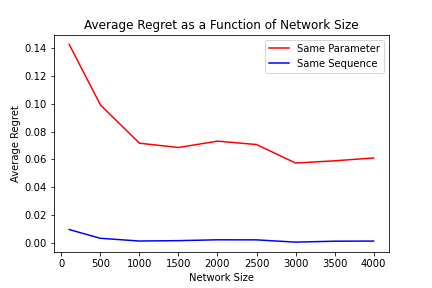
\includegraphics[]{../results/regret_size.png}
  \caption{Regret as a function of n. p is set to $\frac{\sqrt{\log(n)}}{n}$.}
\end{figure}

\subsection{Variance}
Here we plot the variance of regrets of different settings of n and p. At each choice of parameters 15 independent trials are run and when plot the variance of the regret of these trials.
\begin{figure}[h]
  \centering
  \includegraphics[]{../results/var_regret_p.png}
  \caption{Variance of regrets as a function of p. N=1500. At each (n,p) we take the average variance over 15 independent runs.}
\end{figure}

\begin{figure}[h]
  \centering
  \includegraphics[]{../results/var_regret_size.png}
  \caption{{Variance of regrets as a function of n. $p = \frac{\sqrt{\log(n)}}{n}$}}
\end{figure}

\subsection{Closeness to optimal prices}
Yet another question to ask is all the prices being offered via our strategies close to optimal prices. It isn't necessary that the prices of well performing vectors are close to the best vector. We will consider the $\ell_{1}, \ell_{2}, \ell_{\infty}$ differences between the optimal price vector and the vector we generate. For the $\ell_{1}$ and $\ell_{2}$ differences we will compute the average loss per agent.

\begin{figure}[h]
  \centering
  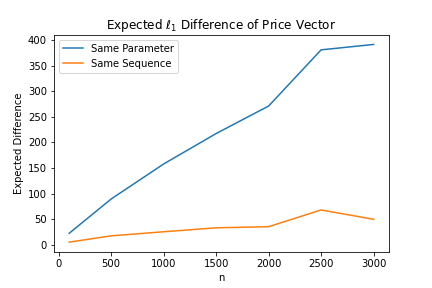
\includegraphics[width=0.4\textwidth]{../results/aprice_vector_l1.png}
  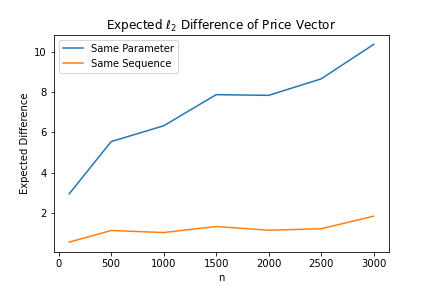
\includegraphics[width=0.4\textwidth]{../results/aprice_vector_l2.png}
  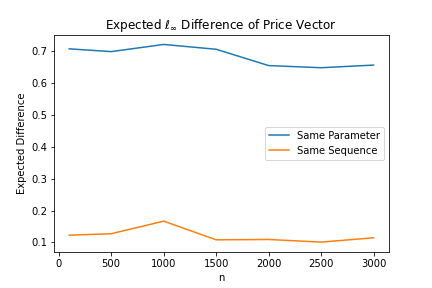
\includegraphics[width=0.4\textwidth]{../results/aprice_vector_inf.png}
  \caption{Difference away from optimal price vector as a function of n. P is $\frac{\sqrt{\log(n)}}{n}$ }
\end{figure}

\begin{figure}[h]
  \centering
  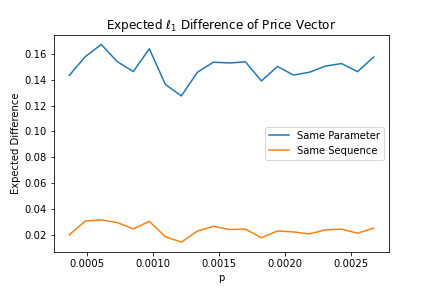
\includegraphics[width=0.4\textwidth]{../results/vdif_vp_l1.png}
  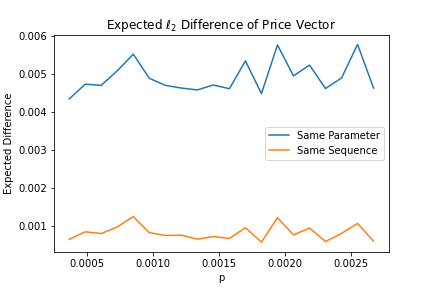
\includegraphics[width=0.4\textwidth]{../results/vdif_vp_l2.png}
  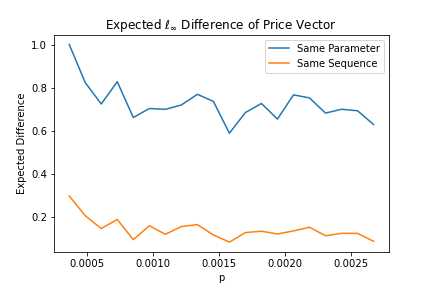
\includegraphics[width=0.4\textwidth]{../results/vdif_vp_inf.png}
  \caption{Difference away from optimal price vector as a function of n. P is $\frac{\sqrt{\log(n)}}{n}$ }
\end{figure}


\subsection{Averaged Vector}
  Here instead of calculating the regret of one price vector here we generate many graphs with the same degree sequence and take the average price vector we obtain.
\begin{figure}[H]
  \centering
  \includegraphics[width=0.8\textwidth]{../results/RegretAveragedVector.png}
  \caption{Regret of using price vector generated graphs generated by the same degree sequence. In the same sequence case we simply take each each graph's price vector and calculate the regret of using the vector. In the averaged case, we can several price vectors and average them together and find the regret of this singular average vector. $p=\frac{\sqrt{\log(n)}}{n}$}
\end{figure}

\subsection{Truncated walks}
This final test is run in a different manner. In the previous tests we generated completely new graphs that had the same degree sequence as the original. There is not an obvious way to generate graphs with the same number of nodes accessible from 2 or more steps starting from a specific  node. Instead we will take our true graph and compute the bonacich centrality but only considering the first k+1 terms of the sum $\sum_{i=0}^{\infty} (\alpha (G+G^{T}))^{i}$. That is only walks of length less than or equal to k  will be considered.


\begin{figure}[H]
  \centering
  \includegraphics[width=0.8\textwidth]{../results/awalk_loss.png}
  \caption{Regret as a function of walk size considered. Here $n=1500$ and $p=\frac{\sqrt{\log(n)}}{n}$ and $\rho=0.99$}
\end{figure}

\section{Conclusion}
From these results we can conclude several things. First we see that generating prices from just any Erdos-Renyi random graph is worse than using the optimal uniform price vector. This is a rather curious result since we expected having some information about the graph to be better than having none. But the other part of our hypothesis turns out to be correct, generating graphs with the degree information yields very low regret price vectors. In addition, it is not only that these price vectors perform well it is also the case they are close to the true optimal price vector. This implies that graphs that are close together, here having the same degree sequence, have respective optimal price vectors are close together. After trying graphs with the same degree sequence we investigated a further strategy of taking the average of these guessed vector. It seems experimentally that this produces half the regret of the previous strategy. Finally, we looked at how much of the price vector is controlled by the information gained from short walks. We found that very short walks carry almost all the information of the Bonacich centrality. This result in particular might be a bit off because the 1-norm is typically notably larger than the 2-norm so it might too small such that higher order terms are essentially 0 in a way that isn't a good model of reality.
\pagebreak

\bibliography{refer}
\bibliographystyle{ieeetr}


\end{document}
